\documentclass{article}
\usepackage[utf8]{inputenc}
\usepackage[margin=1in]{geometry}
\usepackage{amsmath}
\usepackage{hyperref}
\usepackage{epsfig}
\usepackage{array}
\usepackage{graphicx}
\usepackage{color}
\usepackage{textcomp}
\setlength{\parindent}{0em}
\setlength{\parskip}{0.5em}

\title{CTA200H 2023 Assignment 3}
\author{Due by 1:00PM Tuesday May 9}
\date{}

\begin{document}

\maketitle

\section*{Question 1}
I started by defining x and y using np.linspace, making them range from -2 to 2 with 1000 steps. An empty array for c was then made using np.zeros, shaping it to be 1000 by 1000 to fit the dimensions of x and y. X and Y were then defined using np.meshgrid, and c was populated using the equation $c = x + iy$, making c the complex plane.

I then created a function called iterate to iterate the equation: $z_{i + 1} = z_i^2 + c$. This function took the arguments c as described earlier, z0 as the initial z value, and the maximum iteration value: $max \_ iter$. Within this function I created an empty array called $escape \_ iter$, which was populated with the maximum iteration values for which the values of z are greater than some maximum number, in this case 10, indicating that they are unbounded. The iteration value where this happens is then recorded in the $max \_ iter$ array, which the function is designed to return.

The iterate function was then called as a function of c, z0=0, and $max \_ iter=20$, and set equal to sol. This was then plotted using plt.imshow and a color map, where the color scale showed the iteration number at which each respective point in c diverged. This graph had the real part of c on the x-axis and the imaginary part of c on the y axis.  

\begin{figure}
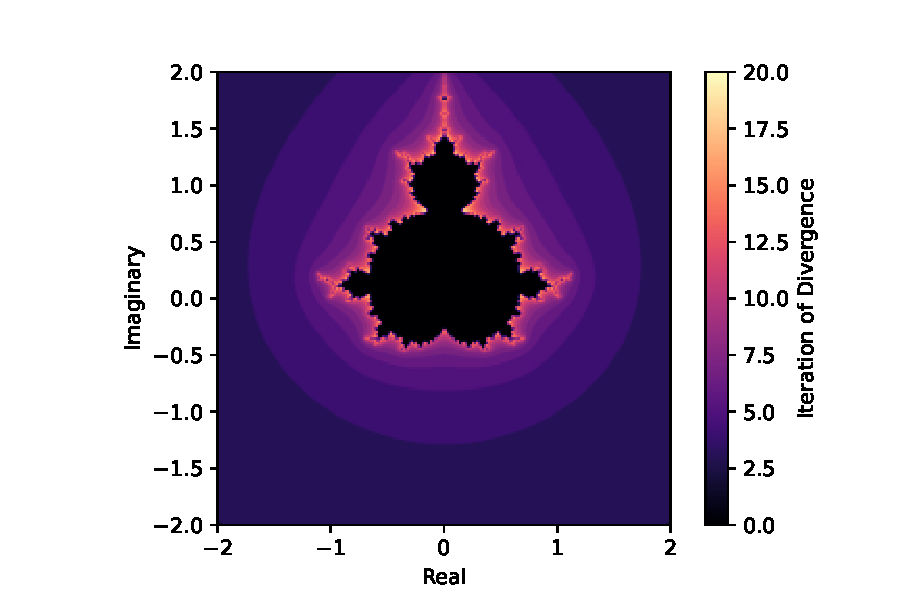
\includegraphics{Q1_2.pdf}
\caption{The plot of c with the colour scale showing the maximum iteration number before the absolute value of z diverges.\vspace{3mm}}
\label{fig:Question1_2}
\end{figure}

An image was then made where the points c that diverge are purple, and the points that remain bound are blue, in Figure 2. This was done by calling the diverging points div and defining them using np.where such that sol<20, and then similarly defining the bound points as bound this defining them such that sol>=20. The bound solutions (sol[bound]) were then set to 1.0, and the diverging solutions (sol[div]) were set to 0. This was done in order to see which points were bound and which diverged when plotting. sol was then plotted using plt.imshow, with the colormap making the diverging points purple and the bound points blue.     

\begin{figure}
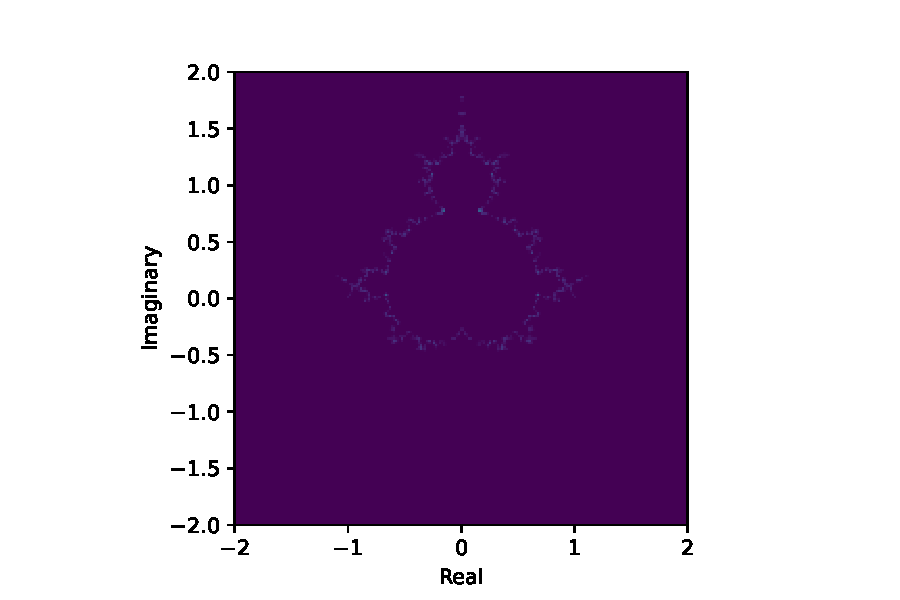
\includegraphics{Q1_1.pdf}
\caption{The plot of c with the the points that remain bound being blue, and the points that diverge being purple.\vspace{3mm}}
\label{fig:Question1_1}
\end{figure}



\section*{Question 2}

First, a function $dW \_ dt$, the derivative of $W\equiv(X, Y, Z)$ was defined using Lorenz equations 25, 26 and 27:
\begin{eqnarray}
\dot X &=& -\sigma(X-Y)\\
\dot Y &=& rX -Y - XZ\\
\dot Z &=& -bZ + XY
\end{eqnarray}

Where sigma is the Prandtl number, r is the Rayleigh number, and b is a dimensionless length scale. This function returned $dW \_ dt$ as a vector, with coordinates \dotX, \dotY, \dotZ. $solve \_ ivp was then used to integrate dW, with the initial conditions $W_0=[0., 1., 0.]$, [$\sigma, r, b$] = [10., 28, 8./3.] for t=60. This was set to be sol. 

Next Lorenz' Figure 1 was recreated, by again solving dW /_ dt, but this time adding the t \_ eval parameter to be a np.linspace going from 0 to 30 with 1000 steps. The second coordinate of the solution W (Y(t)) was then plotted versus the number of iterations, where number of iterations (N) is equal to t/$\Delta t where in this case $\Delta t=0.01$. The plot was then divided into the sections from Lorenz' Figure 1 by plotting v-lines at N=1000, 2000, 3000. This plot can be seen in Figure 3.   

\begin{figure}
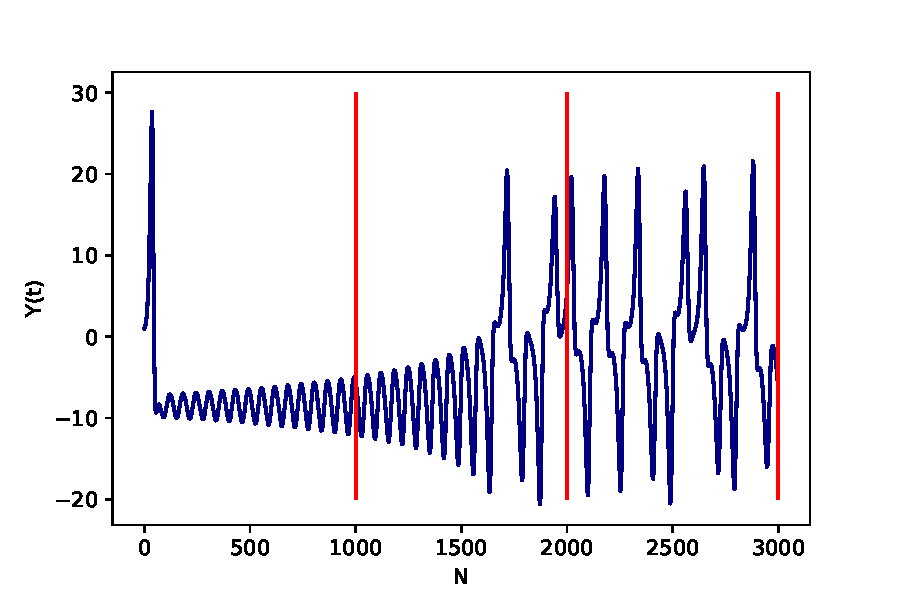
\includegraphics{Q2_1.pdf}
\caption{Recreation of Lorenz' Figure 1, plotting Y(t) versus number of iterations (N).\vspace{3mm}}
\label{fig:LorenzFig1}
\end{figure}


Then Lorenz' Figure 2 was recreated by again solving the ODE, but this time using a different t \_ eval= np.linspace(14, 19, 1000). This two graphs were plotted together, with the first plotting Y(t) versus Z(t), and the second plotting Y(t) versus -X(t). 

Finally the solution to the ODE was calculated again, but this time with the initial conditions slightly varied to $W'_0 = W_0+[0., 1.e-8, 0] = [0., 1.00000001, 0.]$. The distance between W and W' was then calculated by first solving them at the same t=np.linspace[0,10,1000], and then taking the difference by taking the difference between each coordinate in W and W', squaring that value, adding them together and then taking the square root of this value and calling it diff. This was then plotted on a semilog plot, of t versus log of diff. Because the initial conditions were slightly changed, the graph was not linear, instead being oscillatory. This aligns with the fact that Lorenz originally found a linear relation on his semilog plot, implying exponential growth, which aligns with a small change in initial conditions growing rapidly. 


\end{document}
